%%%%%%%%%%%%%%%%%%%%%%%%%%%%%%%%%%%%%%%%%%%%%%%%%%%%%%%
% A template for Wiley article submissions developed by 
% Overleaf for the Overleaf-Wiley pilot which ran 
% during 2017 and 2018.
% 
% This template is no longer supported, but is provided
% for historical reference. Last updated January 2019.
%
% Please note that whilst this template provides a 
% preview of the typeset manuscript for submission, it 
% will not necessarily be the final publication layout.
%
% Document class options:
% =======================
% blind: Anonymise all author, affiliation, correspondence
%        and funding information.
%
% lineno: Adds line numbers.
%
% serif: Sets the body font to be serif. 
%
% twocolumn: Sets the body text in two-column layout. 
% 
% num-refs: Uses numerical citation and references style 
%           (Vancouver-authoryear).
%
% alpha-refs: Uses author-year citation and references style
%             (rss).
%
% Using other bibliography styles:
% =======================
%
% To specify a different bibiography style
%
% 1) Do not use either num-refs or alpha-refs in documentclass.
% 2) Load natbib package with the options set as needed.
% 3) Use the \bibliographystyle command to specify the style
% 
% Included NJD styles are: 
%   WileyNJD-ACS
%   WileyNJD-AMA
%   WileyNJD-AMS
%   WileyNJD-APA
%   WileyNJD-Harvard
%   WileyNJD-VANCOUVER
%
% or you may upload an alternative .bst file 
% (if requested by the journal).
%
% Examples:
% =======================
%% Example: Using numerical, sort-by-authors citations.
\documentclass[alpha-refs,twocolumn]{wiley-article}

%% Example: Using author-year citations and anonymising submission
% \documentclass[blind,alpha-refs]{wiley-article}

%% Example: Using unsrtnat for numerical, in-sequence citations
% \documentclass{wiley-article}
% \usepackage[numbers]{natbib}
% \bibliographystyle{unsrtnat}

%% Example: Using WileyNJD-AMA reference style and superscript
%%          citations, two-column and serif fonts for AIChE
% \documentclass[serif,twocolumn,lineno]{wiley-article}
% \usepackage[super]{natbib}
% \bibliographystyle{WileyNJD-AMA}
% \makeatletter

% \makeatother
\usepackage{lscape}
\usepackage{afterpage}

\usepackage{graphicx}
\usepackage{eso-pic}
\usepackage{stfloats}
\usepackage{float}
\usepackage[section]{placeins}
\usepackage{caption}
\captionsetup[figure]{font=small,labelfont=bf}


% Ajout du logo en haut à droite de la première page
\AddToShipoutPictureBG*{
       \AtPageUpperLeft{%
              \put(\LenToUnit{\paperwidth-4cm},\LenToUnit{-2.6cm}){% Ajustez les coordonnées selon vos besoins
                     
\includegraphics[width=3cm]{Figures/logo-UT.png} % Remplacez 'example-image' par le chemin de votre logo
              }%
       }%
}

\AddToShipoutPictureBG*{
       \AtPageUpperLeft{%
              \put(\LenToUnit{\paperwidth-6.8cm},\LenToUnit{-2.65cm}){% Ajustez les coordonnées selon vos besoins
                     
\includegraphics[width=2.7cm]{Figures/Logo-CRBE.png} % Remplacez 'example-image' par le chemin de votre logo
              }%
       }%
}

\AddToShipoutPictureBG*{
       \AtPageUpperLeft{%
              \put(\LenToUnit{\paperwidth-8cm},\LenToUnit{-2.6cm}){% Ajustez les coordonnées selon vos besoins
                     
\includegraphics[width=1cm]{Figures/LOT.png} % Remplacez 'example-image' par le chemin de votre logo
              }%
       }%
}

\usepackage{xcolor}
\usepackage{hyperref}
\hypersetup{
       colorlinks=true,
       citecolor=blue,
       linkcolor=black,
       urlcolor=blue
}
\usepackage{siunitx}

% Update article type if known
\papertype{Journal of Ecology}
\paperfield{Tropical Ecology}

\title{Composition et assemblage des communautés fongiques chez les plantes épiphytes vasculaires tropicales}

\author[1\authfn{1}]{Mathys Dussel--D'hervé}



\affil[1]{Faculté de Sciences et Ingénieurie - Université de Toulouse III - Paul Sabatier, 118 route de Narbonne, 31062 Toulouse Cedex 9, France}

\corraddress{Céline Leroy, Ecologie des Forêts de Guyane (UMR CNRS 8172), Campus Agronomique, 97379 Kourou Cedex, France}
\corremail{celine.leroy@utoulouse.fr}



\runningauthor{Dussel--D'hervé et al.}
\begin{document}

\begin{frontmatter}
\maketitle

\begin{abstract}
Tropical forests harbor exceptional plant and microbial biodiversity, essential for ecosystem functioning and biogeochemical cycles. Among this diversity, vascular epiphytes are key elements of the canopy, but the composition and assembly of their fungal communities remain poorly understood. This work explores the structure of fungal assemblages associated with different taxonomic groups of epiphytes, comparing roots and leaves, as well as surface (epiphytes) and internal (endophytes) fractions. Based on samples collected in Peru as part of the "Life on Trees" program, fungal communities were characterized by high-throughput metabarcoding of the ITS region. Analyses of alpha and beta diversity, ordination (NMDS), and multivariate tests (PERMANOVA) highlight the influence of microhabitat and host functional strategy on the structuring of fungal niches. These results provide new insights into plant-microorganism interactions within the tropical canopy.

\keywords{Vascular epiphytes, Tropical canopy, Fungal communities, Metabarcoding, ITS, Microbial ecology, Plant-microbe interactions, Biogeochemical cycles}
\end{abstract}
\end{frontmatter}

\section{Introduction}

Fungi play a crucial role in the functioning of terrestrial ecosystems. They drive biogeochemical cycles and directly influence plant dynamics. How are these microbial assemblages structured? It is the result of a complex mix of biotic and abiotic factors, such as temperature or humidity. In tropical environments, which are hotspots of record biodiversity, the links between fungi and host plants take on particular importance \citep{arnold_are_2000, bermudes_fungi_1989}. At the scale of a single plant, the fungal microbiome varies greatly from one organ to another (leaves, roots) and according to its location. We generally distinguish epiphytes, living on the surface, from endophytes, present within tissues. The identity of the plant acts as a selective filter. Through its functional traits, exudates, or immune system, the host shapes its own mycobiome.

To better understand these interactions under extreme constraints, epiphytic plants offer an ideal study model. They represent a huge part of the tropical canopy flora and grow on other trees without parasitizing them \citep{zotz_plants_2016}. This "suspended" lifestyle deprives them of access to the soil. They endure a lack of water and nutrients. To cope with these severe stresses, these plants have had to innovate. They vitally rely on associations with other organisms: animals, bacteria, or fungi. These mutualistic alliances improve their nutrition and help them withstand environmental stress.

Yet, despite such ecological importance, our knowledge of these fungal communities remains very limited. Research has often focused on terrestrial plants, especially those with agronomic value in the tropics, such as coffee or cacao \citep{vega_fungal_2008}. When it comes to epiphytic flora, the situation is similar: studies almost always focus on a few ecological or economic "stars." \textit{Orchidaceae} are the best example, with their near-total dependence on mycorrhizae for germination \citep{dearnaley_orchid_2012}. In contrast, the vast majority of other lineages of neotropical vascular epiphytes remain, from a fungal perspective, a true blind spot to this day.

It is precisely in this context that the \textit{Life on Trees} (LOT) project intervenes, aiming to inventory all eukaryotic biodiversity (animals, plants, fungi, and protists) hosted by a single tropical tree, with a particular focus on fungal communities. Although the study of the mycobiome and its role in adaptation to the extreme conditions of the canopy is central, this project is part of a broader interdisciplinary program. To this end, LOT conducts unprecedented sampling on three giant trees located at different altitudes along the Peruvian Andes (at 400 m, 800 m, and 2500 m), to generate reference data on the assembly of these complex communities.

\section{Materials and Methods}

\subsection{Sampling and bioinformatics}

The three trees studied in the LOT project are distributed along an altitudinal gradient in the Peruvian Andes. This configuration offers a unique opportunity to understand the impact of altitude and local conditions on fungal diversity. The first site, LOT1, is located at about 400 meters above sea level, in the heart of the Amazon. Here, heat and humidity prevail. Higher up, at 800 meters, LOT2 occupies a transition zone at the boundary between lowland tropical forest and the first mountain foothills. Finally, LOT3 peaks at 2500 meters, in the heart of the Andean cloud forest. This last site is characterized by cooler temperatures, persistent humidity, and light filtered by mist.

All these sites are linked to the Wayqecha Biological Station in the Cusco region, managed by the NGO Amazon Conservation. This choice is not accidental: it allows for long-term ecological monitoring and strong research infrastructure. The selected trees belong to different species. LOT1 is a \textit{Dussia tessmannii} (Fabaceae), LOT2 a \textit{Ficus americana subsp. andicola} (Moraceae), and LOT3 a \textit{Brosimum cf. utile} (Moraceae). They serve as hosts to inventory the biodiversity associated with a single tree. By comparing both different sites and various microhabitats within each tree, this approach aims to better understand how environmental gradients and the specific characteristics of each tree influence the structuring of fungal communities in tropical vascular epiphyte plants.

\begin{figure}[htbp]
    \centering
    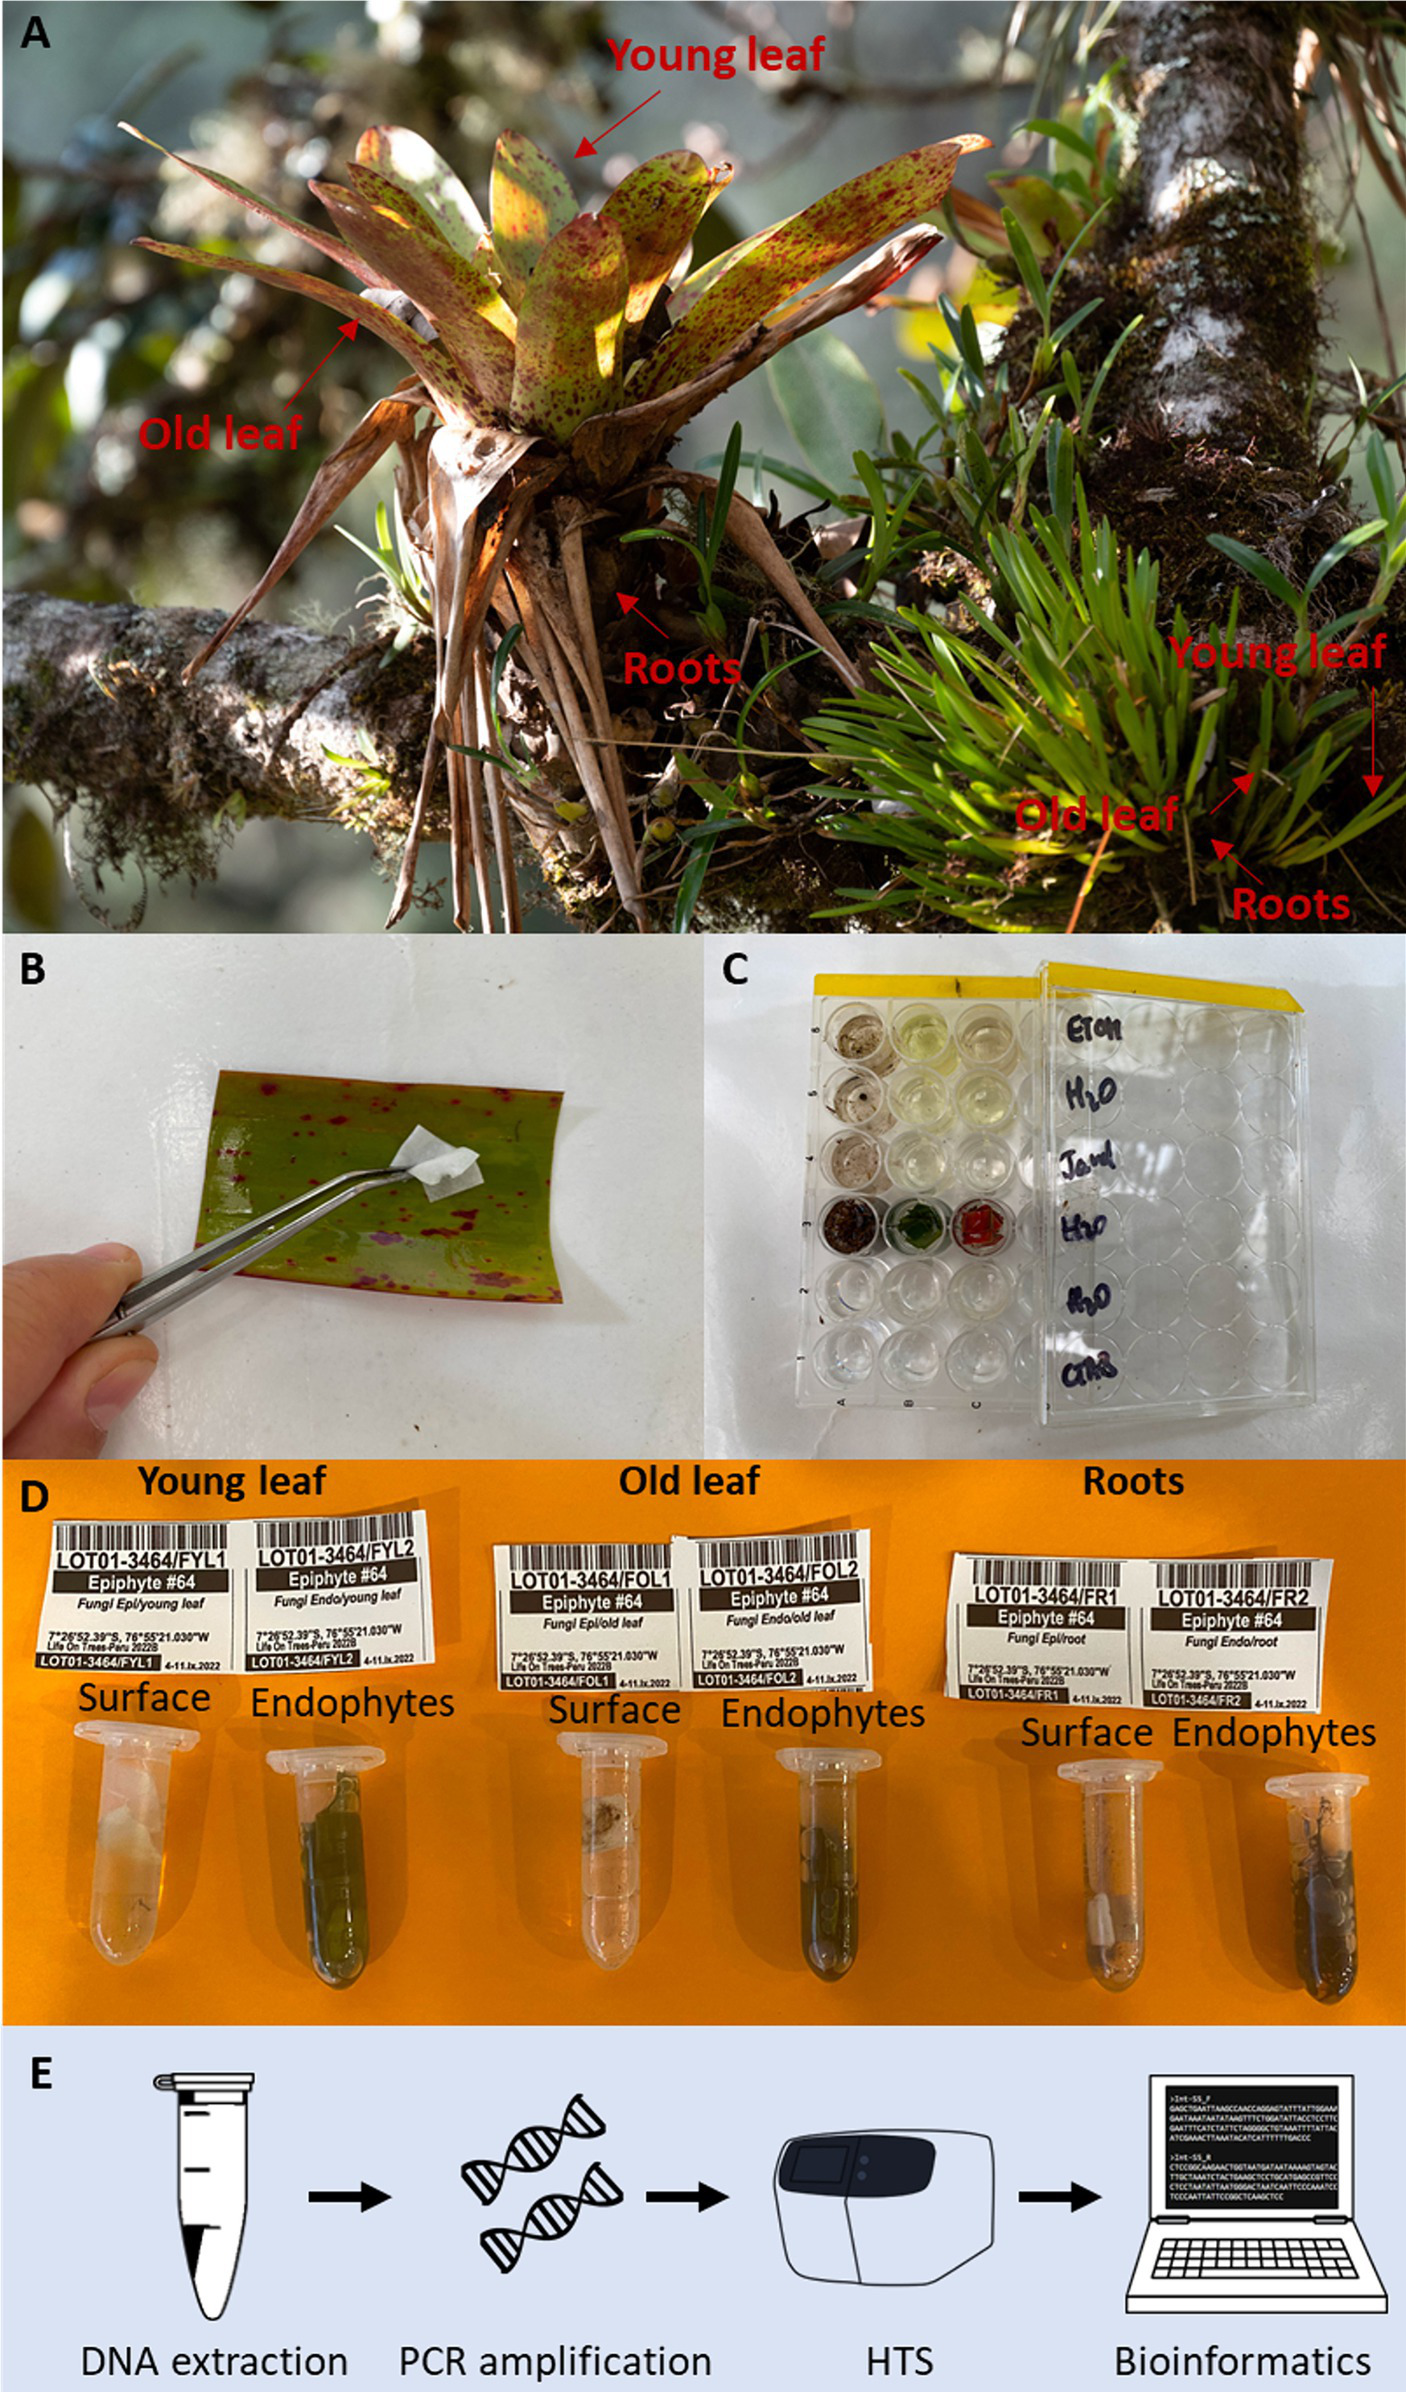
\includegraphics[width=0.9\linewidth]{Figures/sampling_protocol.png}
    \caption[Protocol for isolating surface and endophytic fungi in epiphytic plants.]{
        Procedure for isolating surface and endophytic fungi in epiphytic plants.\\
        {\footnotesize
        (A) For each epiphytic plant individual, a fully developed young leaf, an old leaf, and different parts of the root system were sampled. 
        (B) Sampling of microfungi from the leaf surface was performed using a piece of Whatman paper previously soaked in sterile CTAB buffer. 
        (C) Surface sterilization for endophyte isolation by successively soaking tissue portions in 70\% ethanol, sterile water, 9\% sodium hypochlorite, then washing twice in sterile water, and finally immersing in sterile CTAB buffer. 
        (D) DNA preservation was performed in sterile Eppendorf tubes with CTAB buffer. 
        (E) DNA metabarcoding workflow.\\
        Image credits: (A) Charlie Delhumeau, (B--D) CL. \citep{leponce2024unveiling}
        }
    }
    \label{fig:ma_figure}
\end{figure}

The sampling protocol in this work follows the method described by \citet{leponce2024unveiling}. Fungal communities were studied from previously collected vascular epiphyte plants. For each individual, three compartments were targeted to represent different microhabitats of the host plant: a fully developed young leaf, an old leaf, and several portions of the root system.

Two fungal fractions were then distinguished. Fungi present on the leaf surface were collected by swabbing with a sterile Whatman paper soaked in CTAB buffer. Endophytes were isolated after surface sterilization of plant tissues. This involved successive baths in ethanol, sterile water, and sodium hypochlorite, followed by several rinses before storing the samples in CTAB buffer. This step was essential, as it allowed for distinguishing fungi living on the surface of organs from those present inside the tissues.

The characterization of fungal communities was then based on a high-throughput metabarcoding approach targeting the ITS (Internal Transcribed Spacer) region, commonly used as a reference marker for studying fungal diversity. After PCR amplification, the products were sequenced on an Illumina MiSeq platform. Bioinformatic processing included several successive steps: demultiplexing of reads, quality control, removal of low-quality sequences and chimeras, then clustering into operational taxonomic units (OTUs). Taxonomic assignment was then performed using reference databases adapted to fungi. At the end of this analysis pipeline, a contingency table listing the number of sequences per sample was obtained. All diversity and composition analyses presented here were based on this table \citep{leponce2024unveiling}.

\subsection{Diversity analyses}

To compare alpha diversity, we used Hill numbers, following the approach developed by \citet{chao2014rarefaction}. This method allows for representing both rarefaction (interpolation) and extrapolation of diversity curves. Three orders were considered. The first, \(q=0\), corresponds to species richness. The second, \(q=1\), reflects the effective number of species associated with the Shannon index. Finally, \(q=2\) is based on the Simpson index and gives more weight to dominant taxa. These different indices were then compared between the microhabitats of the host plant—young leaves, old leaves, and roots—as well as between the three sampling sites (LOT1, LOT2, and LOT3).

The curves were generated in \texttt{R} with the \texttt{iNEXT.3D} package \citep{chao2021measuring}. 95\% confidence intervals were estimated by bootstrap from 50 replicates. This analytical framework is particularly useful when sampling effort varies between categories, as it allows for comparing diversity levels on a standardized basis.

We also calculated evenness using Pielou's index, defined as:
\[ J = \frac{H'}{\ln(S)} \]
where \(H'\) is the Shannon index and \(S\) is species richness. This index assesses how evenly abundances are distributed within fungal communities.

\subsection{OTU sharing and relative abundances}

OTU sharing between microhabitats was studied using UpSet diagrams \citep{lex2014upset}. This type of representation is particularly useful for comparing several sets at once and remains more readable than a Venn diagram as the number of categories increases. It allows for identifying OTUs common to several plant compartments, as well as those seemingly specific to a given microhabitat. The graphs were produced in \texttt{R} with the \texttt{UpSetR} package \citep{conway2017upsetr}.

To complement this approach, the most abundant taxa in each microhabitat were summarized in a heatmap. Data were expressed as relative abundances, then transformed into Z-scores (centered and scaled by microhabitat), to compare profiles despite differences in sequencing depth. This representation allows for quickly visualizing dominant OTUs and highlighting composition variations between young leaves, old leaves, and roots. The table was built from OTUs present in at least 5\% of samples in each microhabitat, with the \texttt{pheatmap} package in \texttt{R} \citep{kolde2019pheatmap}. The Z-score is defined as the difference between the observed value and the mean, divided by the standard deviation \citep{altman1991practical}.

These two approaches are complementary. UpSet diagrams describe the degree of OTU sharing between habitats, while the heatmap highlights dominant taxa that contribute most to observed differences between compartments.

\subsection{Similarity analyses}

To study differences in composition between fungal communities, we analyzed beta diversity using a Bray--Curtis dissimilarity matrix calculated on OTU relative abundances \citep{bray1957ordination}. This measure is commonly used for community data, as it incorporates abundance information while being little affected by double absences.

The structure of assemblages was then explored by NMDS (Non-metric Multidimensional Scaling) ordination, performed in \texttt{R} \citep{kruskal1964nonmetric,minchin1987evaluation}. The aim of this approach is to project samples into a low-dimensional space to best reflect the observed similarity relationships between them. The quality of this representation was assessed using the stress value. Values below 0.2 are considered reliable enough for ecological interpretation \citep{kruskal1964nonmetric}.

Finally, differences in composition between groups were tested by PERMANOVA (Permutational Multivariate Analysis of Variance) with the \texttt{adonis2} function from the \texttt{vegan} package \citep{anderson2001new} at 999 permutations. Depending on the dataset, the effects of site (LOT1, LOT2, LOT3) and microhabitat (young leaves, old leaves, roots) were examined separately. Significance was assessed by permutations, and results are presented as \(R^2\), Fisher's pseudo-\(F\) statistic, and \(p\)-value.

\subsection{Fungal niche specialization}

The niche breadth of OTUs was assessed using Levins' index \citep{levins1968evolution}. This index measures how a taxon is distributed among several microhabitats. In practice, it helps distinguish rather generalist OTUs, present in different plant compartments, from more specialized taxa associated with a more limited number of habitats.

For each OTU \(j\), the raw index was calculated as follows:
\[ B_j = \frac{1}{\sum_{i=1}^{n} p_{ij}^{2}} \]
where \(p_{ij}\) is the relative proportion of OTU \(j\) in microhabitat \(i\), and \(n\) is the total number of microhabitats considered. When \(B_j\) is high, it means the OTU is more evenly distributed among the habitats considered and thus has a broader niche.

To make comparisons between taxa more direct, a standardized version of this index was also used:
\[ B_{A} = \frac{B_j - 1}{n - 1} \]
This transformation brings values between 0 and 1. Low values indicate strong specialization, while higher values indicate a more regular occupation of different microhabitats. To avoid rare taxa blurring general trends, the analysis was restricted to the most abundant OTUs. This better highlights the main specialization patterns within fungal communities associated with epiphytic plants.

\section{Results}

\subsection{Alpha diversity analyses}

\begin{figure*}[htbp]
    \centering
    
\includegraphics[width=0.8\textwidth]{Figures/rarefaction_alpha_div.png}
    \caption{Rarefaction and extrapolation curves for alpha diversity (q=0: species richness, q=1: exponential Shannon diversity, and q=2: inverse Simpson diversity) of fungal communities associated with epiphytic plants. Curves are shown for different organs (young leaves, old leaves, roots) or different sites (LOT1, LOT2, or LOT3). 95\% confidence intervals are indicated by shaded areas.}
    \label{fig:inext}
\end{figure*} 

\begin{table*}[htbp]
    \centering
    {\fontsize{8}{9.6}\selectfont
    \renewcommand{\arraystretch}{1.25}
    \setlength{\tabcolsep}{15pt}
    \resizebox{\textwidth}{!}{%
    \begin{tabular}{llllll}
        \hline
        \textbf{Position} & \textbf{Organs} & \textbf{Richness (q0)} & \textbf{Shannon (q1)} & \textbf{Simpson (q2)} & \textbf{Evenness} \\
        \hline
        \multicolumn{6}{l}{\textbf{Diversity by organs and position}} \\
        Epiphytes  & Old leaf   & $1903.132 \pm 4.092$ & $335.264 \pm 0.452$ & $113.957 \pm 0.297$ & 0.18 \\[0.2em]
                   & Root       & $2603.267 \pm 4.366$ & $584.089 \pm 0.442$ & $255.381 \pm 0.287$ & 0.22 \\[0.2em]
                   & Young leaf & $2018.329 \pm 5.493$ & $324.232 \pm 0.387$ & $135.603 \pm 0.229$ & 0.16 \\[0.3em]
        Endophytes & Old leaf   & $2415.849 \pm 6.878$ & $199.032 \pm 0.203$ & $49.380 \pm 0.073$  & 0.08 \\[0.2em]
                   & Root       & $2422.284 \pm 6.803$ & $413.761 \pm 0.228$ & $176.767 \pm 0.162$ & 0.17 \\[0.2em]
                   & Young leaf & $2466.674 \pm 5.309$ & $177.815 \pm 0.221$ & $44.826 \pm 0.078$  & 0.07 \\
        \multicolumn{6}{l}{\textbf{Diversity by projects}} \\
        Projects    & LOT1       & $1680.161 \pm 4.884$ & $381.82 \pm 0.281$  & $102.611 \pm 0.147$ & 0.23 \\[0.2em]
                   & LOT2       & $1753.821 \pm 5.547$ & $290.496 \pm 0.232$ & $110.127 \pm 0.152$ & 0.17 \\[0.2em]
                   & LOT3       & $2031 \pm 5.601$     & $306.332 \pm 0.195$ & $101.155 \pm 0.114$ & 0.15 \\
        \hline
    \end{tabular}%
    }}
    \caption{Alpha diversity of fungal communities by category and assemblage.}
    \label{tab:diversite_alpha}
\end{table*}

The rarefaction and extrapolation curves (figure \ref{fig:inext}) reveal marked contrasts in alpha diversity, both between microhabitats and between sites. The curves for indices \(q=0\), \(q=1\), and \(q=2\) quickly reach a plateau, suggesting that sampling captured the diversity of the most frequent and dominant taxa well.

Comparing the different organs, roots stand out with consistently higher diversity values than leaves for the Shannon and Simpson indices (see table \ref{tab:diversite_alpha}). For surface epiphytes, they show the highest richness (\(2603.267 \pm 4.366\)), as well as the highest Shannon (\(584.089 \pm 0.442\)) and Simpson (\(255.381 \pm 0.287\)) diversities. For endophytes, the species richness (\(q=0\)) of roots (\(2422.284 \pm 6.803\)) is slightly lower than that of young leaves (\(2466.674 \pm 5.309\)), but roots have much higher diversity levels for \(q=1\) (\(413.761 \pm 0.228\)) and \(q=2\) (\(176.767 \pm 0.162\)). In contrast, leaves, especially for endophytes, host less balanced communities dominated by a small number of OTUs.

Differences between young and old leaves vary depending on the fungal fraction considered. For surface epiphytes, old leaves show slightly lower richness than young leaves, but slightly higher Shannon and Simpson diversity. This suggests a more even distribution of abundances. For endophytes, young and old leaves have similar richness (\(\sim 2400{-}2460\) OTUs), but \(q=1\) and \(q=2\) indices remain low, indicating strong dominance by a few taxa. Evenness indices confirm this trend: they are particularly low in endophytic leaves (\(J = 0.07\) to \(0.08\)), while reaching higher values in roots (\(J = 0.17\) to \(0.22\)).

Among sites, LOT3 has the highest species richness (\(2031 \pm 5.601\)), while LOT1 stands out for the highest Shannon diversity (\(381.82 \pm 0.281\)) and best evenness (\(J = 0.23\)). LOT2 has intermediate richness and the highest Simpson diversity (\(110.127 \pm 0.152\)). However, differences between sites are less pronounced than those observed between organs. Overall, these results show that microhabitat, especially the root/leaf contrast, shapes alpha diversity of fungal communities more strongly than the site's geographic location.

\subsection{OTU sharing and relative abundances}

\begin{figure*}[htbp]
    \centering
    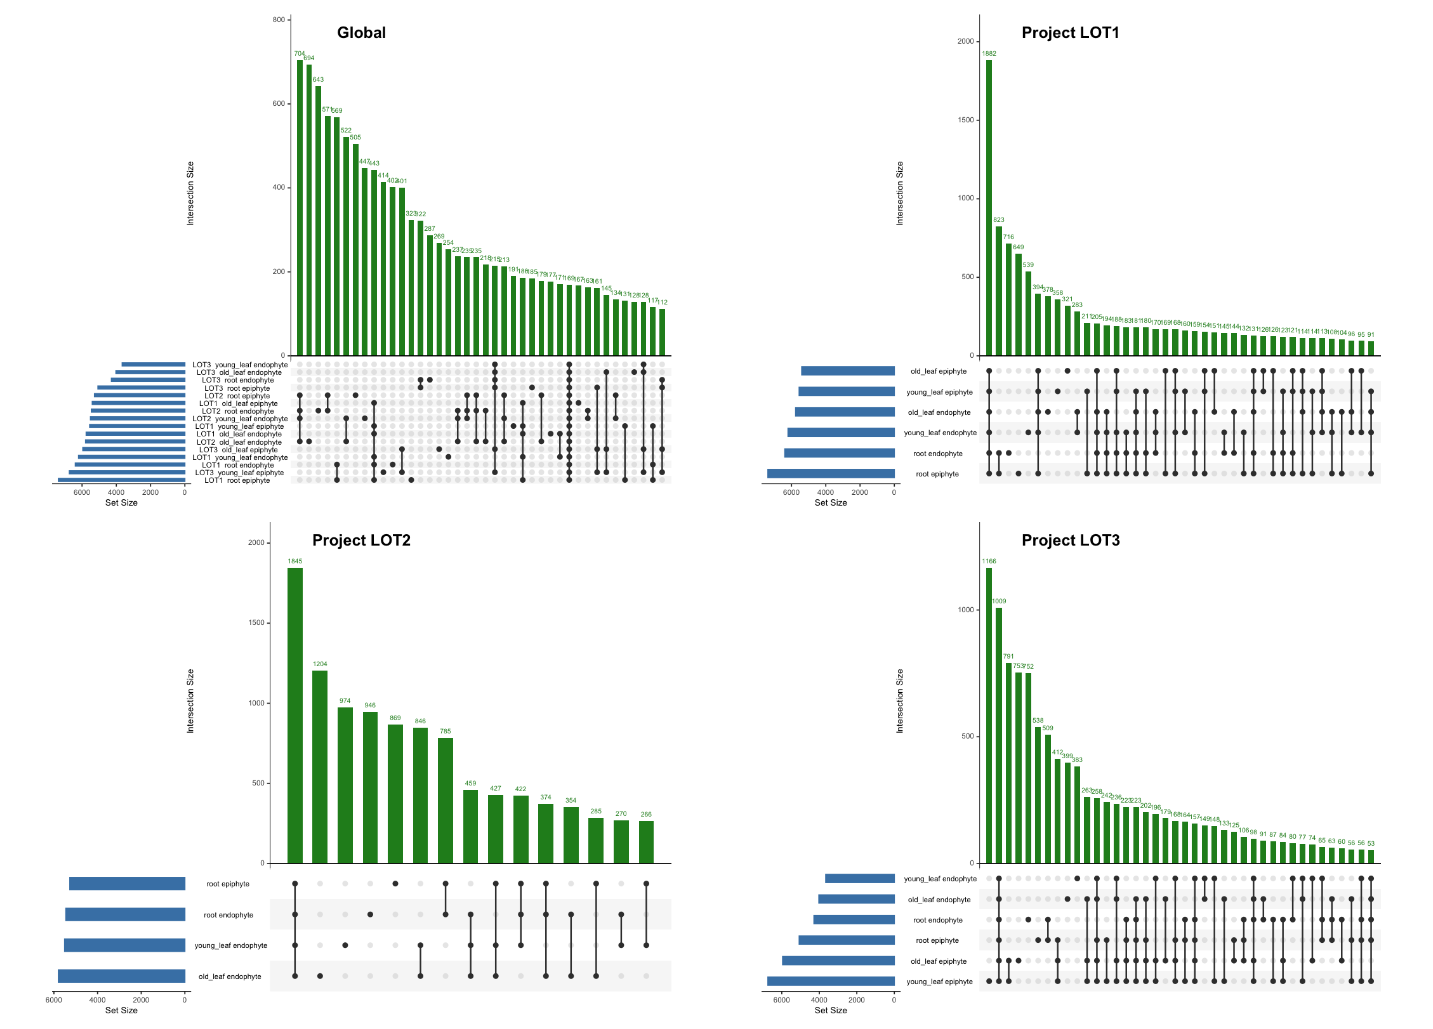
\includegraphics[width=0.8\textwidth]{Figures/upset_plots.png}
    \caption{UpSet diagrams for OTUs shared between microhabitats.}
    \label{fig:upset}
\end{figure*}

The UpSet diagrams (figure \ref{fig:upset}) illustrate the distribution of OTUs among different microhabitats. A core of OTUs is shared by several compartments, but a large part of the diversity remains specific to each organ. Roots, in particular, stand out with a high number of exclusive OTUs. This reflects an original fungal composition, distinct from that of leaves. In contrast, young and old leaves share more of their communities, suggesting ecological proximity between these two tissue types.

This finding matches the alpha diversity results, which already showed particularly high richness in roots. It seems that this microhabitat is both a refuge for specialized taxa and a meeting point for more generalist species. Leaves, meanwhile, host more similar assemblages, probably due to similar environmental and physiological conditions.

In summary, the distribution of fungal OTUs appears strongly structured by microhabitat. Differences between belowground and aboveground organs are clear, and the role of the root compartment as a reservoir of diversity is confirmed by these analyses.

\begin{figure}[htbp]
    \centering
    \includegraphics[width=0.9\linewidth]{Figures/heatmap_orders.png}
    \caption{Heatmap of the most abundant OTUs in each microhabitat.}
    \label{fig:abondances}
\end{figure}

The heatmap of the most abundant OTUs (figure \ref{fig:abondances}) clearly illustrates how much community composition varies from one microhabitat to another. Roots, for example, stand out: they host a set of dominant OTUs that largely differ from those found in leaves. This contrast highlights the strong structuring of fungal assemblages according to the organ studied. In contrast, young and old leaves show more similar abundance profiles, with several common dominant OTUs, even if their relative abundance sometimes varies significantly between compartments.

It is also noticeable that the distribution of dominant taxa is not homogeneous. Some OTUs seem almost exclusive to a single microhabitat, suggesting a particular affinity for specific local conditions. Others, on the contrary, are present in several compartments, but their relative importance fluctuates greatly depending on the organ. This organization shows that differences between organs are not only based on the presence or absence of certain taxa, but also on changes in the abundance hierarchy among shared OTUs.

Overall, these observations match the results of the UpSet diagrams and alpha diversity analyses. Roots appear as an original reservoir of diversity, while leaves share more of their dominant taxa. Thus, the microhabitat within the host plant emerges as a key factor, both for the composition and abundance structure of fungal communities.

\subsection{Similarity analyses}

The NMDS ordination (figure \ref{fig:nmds}) reveals a clear structuring of fungal communities, both by sampling site and microhabitat (see table \ref{tab:permanova_nmds}). At the global scale (panel A), samples tend to cluster according to the LOT project, reflecting a site effect on assemblage composition. PERMANOVA confirms this trend (\(R^2 = 0.108\), pseudo-\(F = 69.483\), \(p = 0.010\)), although a large part of the variation is shared between sites.

When examining each project separately (panels B to D), structuring by organ also becomes very marked. In all three sites, roots form a distinct group, well separated from leaves, while young and old leaves overlap more. PERMANOVA tests show a significant effect of organ in LOT1 (\(R^2 = 0.079\), \(F = 17.802\), \(p = 0.001\)), LOT2 (\(R^2 = 0.085\), \(F = 12.716\), \(p = 0.010\)), and LOT3 (\(R^2 = 0.086\), \(F = 19.752\), \(p = 0.010\)).

The stress values of the ordinations, between \(0.136\) and \(0.150\), are well below the 0.2 threshold, ensuring a faithful representation of dissimilarity relationships between samples. In summary, these analyses show that the composition of fungal communities varies not only between Andean sites, but also, and above all, between different organs of the host plant. The effect of microhabitat thus appears particularly decisive in structuring these assemblages.

\begin{figure*}[htbp]
       \centering
       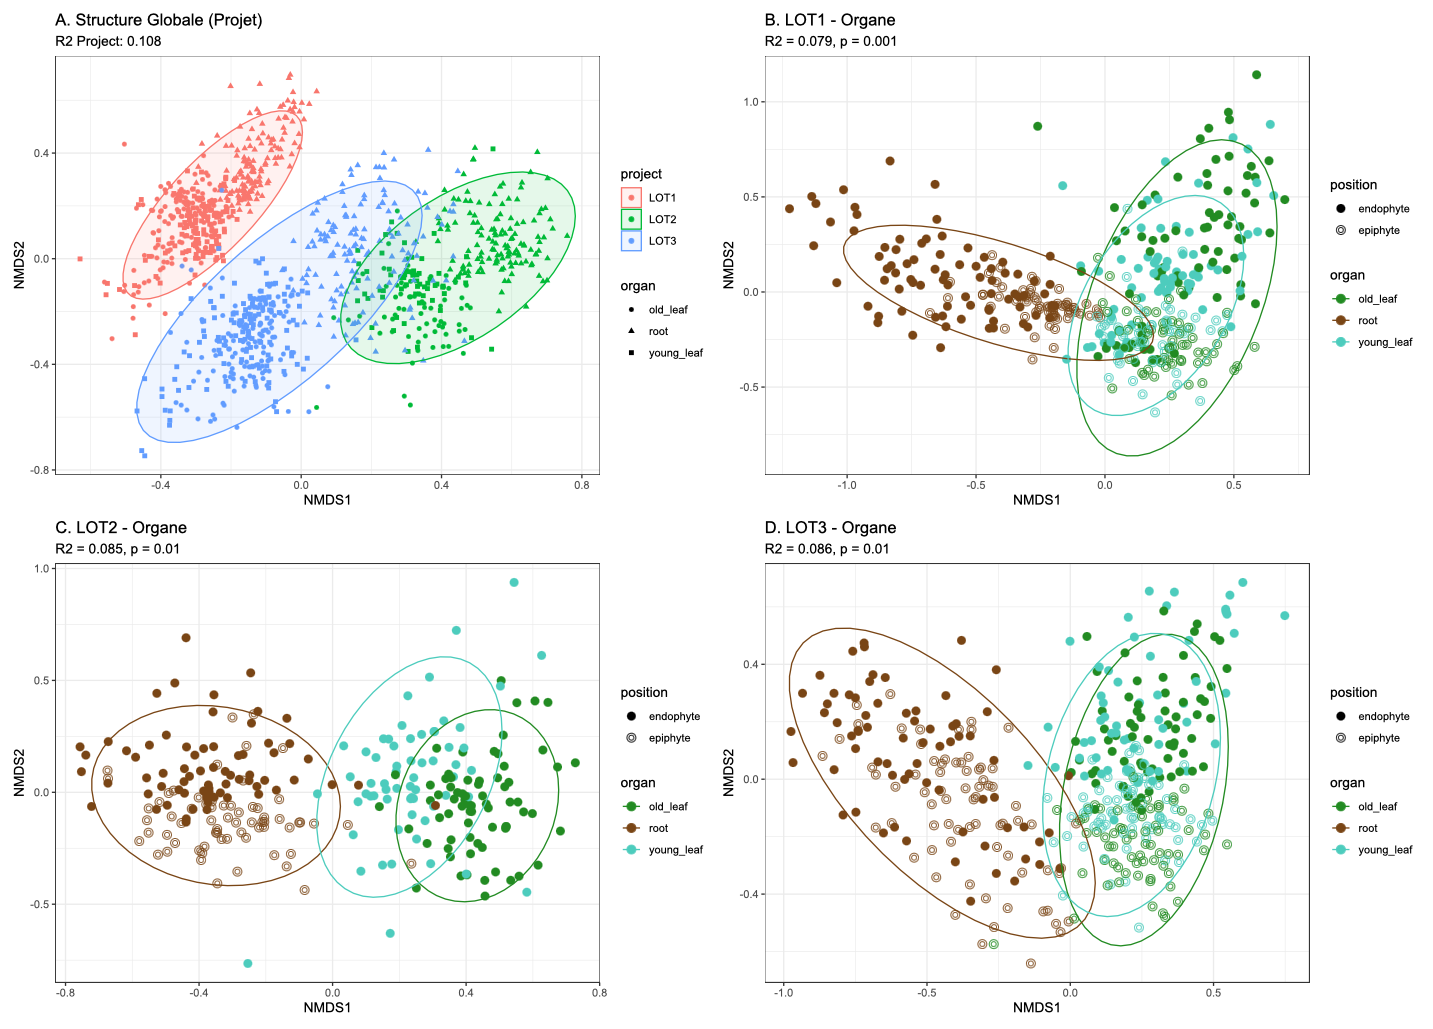
\includegraphics[width=0.8\textwidth]{Figures/NMDS.png}
       \caption{NMDS ordination of fungal communities associated with epiphytic plants.}
       \label{fig:nmds}
\end{figure*}

\begin{table*}[htbp]
       \centering
       \caption{Results of fungal community structure analyses by NMDS and PERMANOVA according to the panels presented in figure \ref{fig:nmds}.}
       \label{tab:permanova_nmds}
       \vspace{0.5cm}
       \renewcommand{\arraystretch}{1.2}
       \setlength{\tabcolsep}{8pt}
       \resizebox{\textwidth}{!}{%
       \begin{tabular}{llllllllll}
              \hline
              \textbf{Panel} & \textbf{Analysis} & \textbf{Tested effect} & \textbf{Samples} & \textbf{Df} & \textbf{R\textsuperscript{2}} & \textbf{F} & \textbf{p-value} & \textbf{Significance} & \textbf{NMDS Stress} \\
              \hline
              A & Global structure (Project) & Project & 1075 & 2 & 0.108 & 69.483 & 0.001 & ** & 0.136 \\
              B & LOT1 -- Organ             & Organ & 402  & 2 & 0.079 & 17.802 & 0.001 & ** & 0.150 \\
              C & LOT2 -- Organ             & Organ & 267  & 2 & 0.085 & 12.716 & 0.001 & ** & 0.148 \\
              D & LOT3 -- Organ             & Organ & 406  & 2 & 0.086 & 19.752 & 0.001 & ** & 0.149 \\
              \hline
       \end{tabular}%
       }
\end{table*}

\subsection{Fungal niche specialization}

Examining Levins' index values (figure \ref{fig:niches_levins}) highlights a wide range of niche breadths among dominant OTUs. Many taxa show low to intermediate scores, indicating uneven distribution among different microhabitats and suggesting some specialization. Conversely, a few OTUs stand out with much higher values, characteristic of generalist behavior and a more balanced presence in several plant compartments.

Dominant OTUs found in roots particularly illustrate this specialization phenomenon. Several of them seem almost exclusively associated with this microhabitat, confirming that roots harbor a unique set of fungi adapted to specific conditions. This finding echoes previous results, which already showed high richness and unique composition in this compartment.

For leaves, whether young or old, dominant OTUs most often have intermediate niche breadths. This suggests that these two tissue types share part of their fungal assemblage, without being identical. The ecological conditions of leaves, though similar, allow some taxa to settle in both compartments, while others remain more faithful to a particular leaf stage.

In sum, Levins' index analysis highlights a non-random organization of fungal communities within the host plant. There is a coexistence of specialists, mainly confined to one microhabitat, and generalists able to occupy several compartments. This pattern confirms the central role of microhabitat as an ecological filter in assembling fungal communities associated with epiphytic plants.

\begin{figure}[htbp]
    \centering
    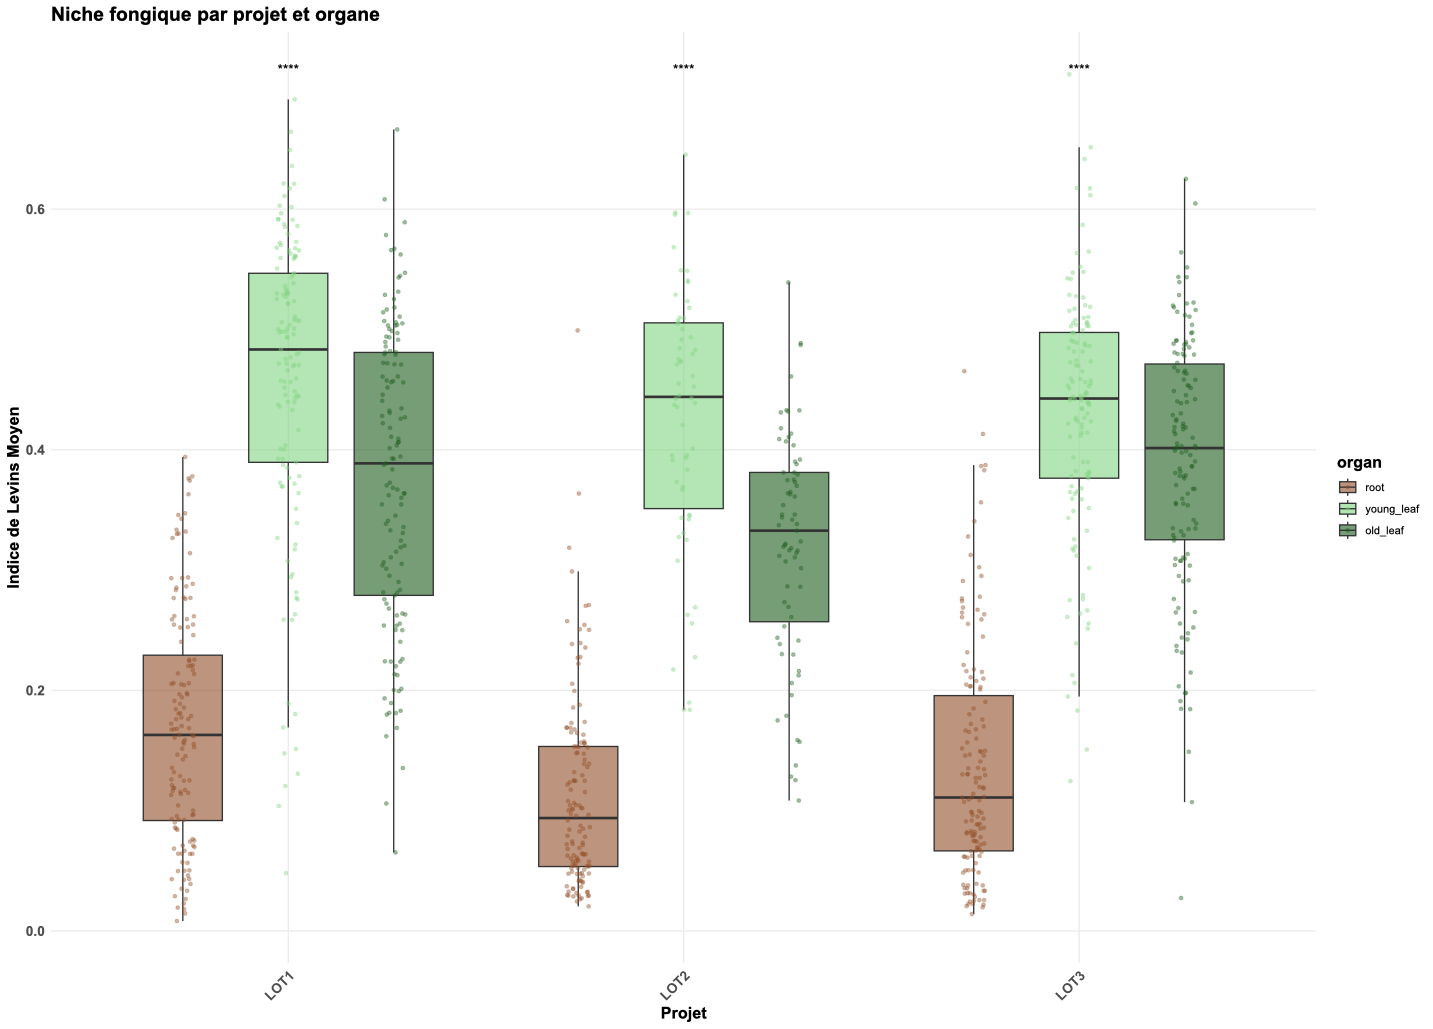
\includegraphics[width=1\linewidth]{Figures/niches_de_levins.png}
    \caption{Levins' index for the most abundant OTUs in each microhabitat.}
    \label{fig:niches_levins}
\end{figure}
\FloatBarrier

\section{Discussion}

The structuring of fungal communities in tropical epiphytic plants highlights the major influence of microhabitat on the diversity and composition of assemblages. Our results show that roots, whether surface or endophytic, host not only the greatest species richness but also the most diverse and even communities. This finding matches observations in other tropical systems, where roots often constitute a reservoir of microbial diversity, probably due to their central role in resource acquisition and the complexity of their immediate environment.

In contrast, leaves, especially when considering the endophytic fraction, present communities dominated by a small number of taxa. This low evenness could reflect stricter selection by leaf tissues, which impose strong physiological and chemical constraints. It is interesting to note that young and old leaves share part of their fungal assemblage but also retain specificities, suggesting that leaf developmental stage modulates community assembly.

OTU sharing between microhabitats, revealed by UpSet diagrams, confirms the existence of a core of generalist taxa able to colonize several plant compartments. However, most OTUs remain specific to a given organ, particularly in roots. This specialization is corroborated by Levins' index, which highlights the coexistence of specialists and generalists among dominant communities. This assembly pattern, where microhabitat acts as a strong ecological filter, is consistent with current models of plant microbiome structuring.

Similarity analyses (NMDS and PERMANOVA) also emphasize the importance of sampling site, even if its effect is less marked than that of microhabitat. Differences between the three studied trees may reflect local variations in climate, substrate, or epiphytic flora composition. Nevertheless, the clearest structuring is always observed between organs, suggesting that internal plant constraints outweigh external environmental factors.

These results open several perspectives. First, they invite further study of functional interactions between fungi and epiphytes, especially to understand how fungal niche specialization contributes to plant adaptation to the extreme conditions of the canopy. Next, they highlight the need to extend analyses to other functional groups (bacteria, protists) and other tropical regions, to test the generality of the patterns observed here.

Finally, this work highlights the relevance of metabarcoding approaches and multivariate analyses for deciphering the complexity of microbial communities associated with plants. It shows that, even in environments as rich and little explored as the tropical canopy, it is possible to identify robust assembly rules governed by the host's internal structure and the ecological specialization of microorganisms. This knowledge is essential for better understanding the functioning of tropical ecosystems and anticipating their response to global changes.

\bibliography{BIBLIO_Stage_LOT_CRBE.bib}



\end{document}